%%%%%%%%%%%%%%%%%%% vorlage.tex %%%%%%%%%%%%%%%%%%%%%%%%%%%%%
%
% LaTeX-Vorlage zur Erstellung von Projekt-Dokumentationen
% im Fachbereich Informatik der Hochschule Trier
%
% Basis: Vorlage svmono des Springer Verlags
%
%%%%%%%%%%%%%%%%%%%%%%%%%%%%%%%%%%%%%%%%%%%%%%%%%%%%%%%%%%%%%

\documentclass[envcountsame,envcountchap, deutsch]{i-studis}

\usepackage{makeidx}         	% Index
\usepackage{multicol}        	% Zweispaltiger Index
%\usepackage[bottom]{footmisc}	% Erzeugung von Fu�noten

%%-----------------------------------------------------
%\newif\ifpdf
%\ifx\pdfoutput\undefined
%\pdffalse
%\else
%\pdfoutput=1
%\pdftrue
%\fi
%%--------------------------------------------------------
%\ifpdf
\usepackage[pdftex]{graphicx}
\usepackage[pdftex,plainpages=false]{hyperref}
%\else
%\usepackage{graphicx}
%\usepackage[plainpages=false]{hyperref}
%\fi


%%-----------------------------------------------------
\usepackage{color}				% Farbverwaltung
%\usepackage{ngerman} 			% Neue deutsche Rechtsschreibung
\usepackage[english, ngerman]{babel}
%\usepackage[latin1]{inputenc} 	% Erm�glicht Umlaute-Darstellung
\usepackage[utf8]{inputenc}  	% Erm�glicht Umlaute-Darstellung unter Linux (je nach verwendetem Format)

%-----------------------------------------------------
\usepackage{listings} 			% Code-Darstellung
\lstset
{
	basicstyle=\scriptsize, 	% print whole listing small
	keywordstyle=\color{blue}\bfseries,
								% underlined bold black keywords
	identifierstyle=, 			% nothing happens
	commentstyle=\color{red}, 	% white comments
	stringstyle=\ttfamily, 		% typewriter type for strings
	showstringspaces=false, 	% no special string spaces
	framexleftmargin=7mm, 
	tabsize=3,
	showtabs=false,
	frame=single, 
	rulesepcolor=\color{blue},
	numbers=left,
	linewidth=146mm,
	xleftmargin=8mm
}
\usepackage{textcomp} 			% Celsius-Darstellung
\usepackage{amssymb,amsfonts,amstext,amsmath}	% Mathematische Symbole
\newtheorem{definition}{Definition}
\newtheorem{satz}{Satz}
\newtheorem{beweis}{Beweis}
\usepackage[german, ruled, vlined]{algorithm2e}
\usepackage[a4paper]{geometry} % Andere Formatierung
\usepackage{bibgerm}
\usepackage{array}
\usepackage{framed}
\hyphenation{Schluss-fol-ger-ungs-sys-tem} 		% Weitere Silbentrennung bei Bedarf angeben
\setlength{\textheight}{1.1\textheight}
\pagestyle{myheadings} 			% Erzeugt selbstdefinierte Kopfzeile

\makeindex 						% Index-Erstellung


%--------------------------------------------------------------------------
\begin{document}
%------------------------- Titelblatt -------------------------------------
\title{Konzeption und Implementierung eines Schlussfolgerungssystems für Hornlogik mit einer funktionalen Programmiersprache}
\subtitle{}
%---- Die Art der Dokumentation kann hier ausgew�hlt werden---------------
%\project{Bachelor-Projektarbeit}
%\project{Bachelor-Abschlussarbeit}
%\project{Master-Projektstudium}
\project{Master-Abschlussarbeit}
%\project{Seminar zur Vorlesung ...}
%\project{Hausarbeit zur Vorlesung ...}
%--------------------------------------------------------------------------
\supervisor{Prof. Dr. Karl Hans Bläsius} 		% Betreuer der Arbeit
\author{Steven Kutsch} 							% Autor der Arbeit
\address{Trier,} 							% Im Zusammenhang mit dem Datum wird hinter dem Ort ein Komma angegeben
\submitdate{27.8.2015} 				% Abgabedatum
%\begingroup
%  \renewcommand{\thepage}{title}
%  \mytitlepage
%  \newpage
%\endgroup
\begingroup
  \renewcommand{\thepage}{Titel}
  \mytitlepage
  \newpage
\endgroup
%--------------------------------------------------------------------------
\frontmatter 
%--------------------------------------------------------------------------
%\preface

Ein Vorwort ist nicht unbedingt n�tig. Falls Sie ein Vorwort schreiben, so ist dies der Platz, um z.B. die Firma vorzustellen, in der diese Arbeit entstanden ist, oder einigen Leuten zu danken, die in irgendeiner Form positiv zur Entstehung dieser Arbeit beigetragen haben. Auf keinen Fall sollten Sie im Vorwort die Aufgabenstellung n�her erl�utern oder vertieft auf technische Sachverhalte eingehen.				% Vorwort (optional)
\kurzfassung

Entwickelt wurde ein Schlussfolgerungssystem für Hornlogik basierend auf der SLD-Resolution. Logikprogramme werden aus einer Textdatei geparst und in eine interne Repräsentation überführt. Auf Basis dieser internen Repräsentation wurden die Unifikation von Literalen sowie ein Resolutionsverfahren nach SLD-Strategie implementiert. Das System wurde in Lisp implementiert. Die Arbeit beschreibt nötige Grundlagen der Logik sowie das Vorgehen bei Entwurf und Implementierung.
 			% Kurzfassung Deutsch/English
\tableofcontents 						% Inhaltsverzeichnis
%\listoffigures 							% Abbildungsverzeichnis (optional)
%\listoftables 							% Tabellenverzeichnis (optional)
%--------------------------------------------------------------------------
\mainmatter                        		% Hauptteil (ab hier arab. Seitenzahlen)
%--------------------------------------------------------------------------
% Die Kapitel werden in separaten .tex-Dateien abgelegt und hier eingebunden.
\chapter{Einleitung}
Schlussfolgerungssysteme entscheiden, ob eine Aussage aus einer Menge von Axiomen folgt. Sie stellen damit eine unmittelbare Anwendung der formalen Logik dar und sind der Kern logischer Programmiersprachen. Als Inferenzmaschinen finden sie Anwendung in der künstlichen Intelligenz.

Aufgrund ihrer Relevanz für praktische Anwendungen sind Schlussfolgerungssysteme in Form der logischen Programmiersprache Prolog Teil der Lehrveranstaltung Angewandte Logik. Den Studenten sollen Grundlagen der logischen und symbolischen Programmierung sowie das Prinzip der Rekursion näher gebracht werden. Nicht logische Bestandteile von Prolog sind nicht Inhalt der Lehrveranstaltung.

Als Alternative für Prolog sollte ein Schlussfolgerungssystem entwickelt werden, das den Fokus auf logische und symbolische Programmierung anstatt auf praktische Relevanz legt. Es sollte einfacher sein, den Zusammenhang zwischen Formeln und Logik-Programmen und so die Relevanz der theoretischen Inhalte der Lehrveranstaltung zu erkennen.

Zu diesem Zweck soll in dieser Arbeit die formale Sprache CL-Reason entwickelt werden, die Nähe zur klassischen Darstellung von Formeln mit dem syntaktischen Komfort von Prolog verbindet. Für diese Sprache wird ein Parser entwickelt, mit dessen Hilfe es möglich ist, Formeln in eine interne Repräsentation zu überführen. Auf dieser internen Repräsentation der Formeln ist nun das automatisierte Durchführen von Schlussfolgerungen gemäß der in der Lehrveranstaltung vorgestellten Techniken möglich.

Die Arbeit behandelt Grundlagen der formalen Logik (Kapitel \ref{logik}) und für Konzeption und Implementierung wichtige Erkenntnisse aus dem logischen Kern der Programmiersprache Prolog (Kapitel \ref{prolog}). Schließlich wird das Vorgehen bei der Konzeption (Kapitel \ref{konzeption}) und der Implementierung (Kapitel \ref{implementierung}) beschrieben. Ein Ausblick beschreibt denkbare und sinnvolle Erweiterungen des entwickelten Systems (Kapitel \ref{ausblick}).

\chapter{Logische Grundbegriffe}\label{logik}

In diesem Kapitel sollen die für spätere Ausführungen benötigten Grundbegriffe der formalen Logik (insbesondere der Prädikatenlogik) eingeführt werden. Dabei soll auf Syntax und Semantik der Prädikatenlogik, Hornklauseln, Unifikation und Resolutionsverfahren sowie -strategien eingegangen werden.

\section{Prädikatenlogik}\label{praedlog}
Die Prädikatenlogik ist eine Erweiterung der Aussagenlogik, bei der Literale nicht als Aussagen mit einem fixen Wahrheitswert interpretiert werden, sondern als Prädikate, deren Wahrheitswert von ihren Argumenten abhängt. In diesem Abschnitt werden Syntax und Semantik der Prädikatenlogik eingeführt. Die hier verwendete Darstellung von Formeln ist umfangreicher in \cite{beckstein} zu finden.

\subsection{Syntax}
Formeln der Prädikatenlogik sind Wörter über dem Alphabet

\begin{equation}
  \Sigma = V \cup F \cup P \cup J \cup Q \cup I
\end{equation}
wobei

\begin{itemize}
\item $V = \left \{ x_{1},...,x_{n} \right \}$ (Variablensymbole),
\item $F$ eine Menge von n-stelligen Funktionssymbolen (einschließlich von 0-stelligen Funktionen, den sog. Konstanten),
\item $P$ eine Menge von n-stelligen Prädikatssymbolen,
\item $J = \left \{ \neg , \wedge , \vee , \Rightarrow ,\Leftrightarrow   \right \}$ (Junktoren),
\item $Q = \left \{ \exists , \forall \right \}$ (Quantoren),
\item $I = \left \{ :, , , (, )\rigth \}$ (Interpunktionen)
\end{itemize}
\noindent
sind.

Prädikatesymbole und Funktionssymbole bilden die Signatur einer prädikatenlogischen Sprache. Sie sind von der Anwendung abhängig und müssen disjunkt sein. Alle Funktions- oder Prädikatsymbole müssen von den in den anderen Teilmengen vorkommenden Symbolen verschieden sein.

Aus Variablen, Konstanten und Funktionssymbolen lassen sich Terme bilden.

\begin{leftbar}
  \begin{definition}[Terme]\label{terme}
    \begin{description}
    \item[(IA)] Variablen und Konstantensymbole sind Terme \newline
    \item[(IS)] Sind $t_{1},...,t_{n}$ Terme und $f$ ein Funktionssymbol, ist auch $f(t_{1},...,t_{n})$ ein Term.
    \end{description}
  \end{definition}
\end{leftbar}
\noindent
Aus Termen und einem Prädikatsymbol lassen sich atomare Formeln bilden.

\begin{leftbar}
  \begin{definition}[atomare Formel]
    \newline
    Seien  $t_{1},...,t_{n}$ Terme und $P$ ein Prädikatssymbol. Dann ist $P(t_{1},...,t_{n})$ eine atomare Formel. Wir nennen atomare Formeln auch kurz Atome    
  \end{definition}
\end{leftbar}
\noindent
Durch das Verknüpfen von atomaren Formeln mittels Junktoren und das Quantifizieren von Variablen lassen sich zusammengesetzte Formeln bilden.

\begin{leftbar}
  \begin{definition}[Formeln]
    \begin{description}
    \item[(IA)] Atomare Formeln sind Formeln \newline
    \item[(IS)] Sind $F$ und $G$ Formeln und $x_{1},...,x_{n}$ Variablen, dann sind auch
      \begin{itemize}
      \item $\neg F$ (Negation),
      \item $F \wedge G$ (Konjunktion),
      \item $F \vee G$ (Disjunktion),
      \item $F \Rightarrow G$ (Implikation),
      \item $F \Leftrightarrow G$ (Äquivalenz),
      \item $\forall x_{1},...,x_{n}:F$ und
      \item $\exists x_{1},...,x_{n}:F$
      \end{itemize}
      Formeln.
    \end{description}
  \end{definition}
\end{leftbar}
\noindent
Mit diesen drei Definitionen lassen sich alle Formeln der Prädikatenlogik bilden. Der Begriff des Literals erlaubt uns für die folgenden Ausführungen eine kompaktere Darstellung von Formeln.

\begin{leftbar}
  \begin{definition}[Literal]
    \newline
    Ein Literal ist eine atomare Formel (positives Literal) oder eine negierte atomare Formel (negatives Literal).
  \end{definition}
\end{leftbar}

Das in dieser Arbeit entwickelte Schlussfolgerungssystem arbeitet auf einer bestimmten Teilmenge prädikatenlogischer Formeln, die als Hornklauseln bezeichnet werden. Wir betrachten zunächst die allgemeine Darstellung prädikatenlogischer Formeln als Menge von Klauseln.

\begin{leftbar}
  \begin{definition}[Konjunktive und Klauselnormalform]
    \newline
    Eine Formel ist in konjunktiver Normalform, wenn sie nur aus einer Konjunktion von Disjunktionen von Literalen besteht.
    \newline
    Sind $L_{11},...,L_{mn}$ Literale (für $m,n \geq 1$) ist die Formel
    \begin{equation}
      ((L_{11} \vee ... \vee L_{1n}) \wedge ... \wedge (L_{m1} \vee ... \vee L_{mn}))
    \end{equation}
    in konjunktiver Normalform.
    \newline
    Die Klauselnormalform ist eine Mengendarstellung einer Formel in konjunktiver Normalform.
    \begin{equation}
      \left \{ \left \{L_{11},...,L_{1n}\right \},...,\left \{ L_{m1},...,L_{mn}\right \} \right \}
    \end{equation}
    \newline
    Ein Element der Klauselnormalform nennen wir Klausel.
  \end{definition}
\end{leftbar}
\noindent
Jede prädikatenlogische Formel lässt sich in eine erfüllbarkeitsäquivalente Formel in Klauselnormalform überführen.

\begin{leftbar}
  \begin{definition}[Hornklausel]
    \newline
    Eine Hornklausel ist eine Klausel die höchstens ein positives Literal enthält.
  \end{definition}
\end{leftbar}
\noindent
Hornklauseln lassen sich auf zwei verschiedene Arten bequem als prädikatenlogische Formeln darstellen.

\begin{leftbar}
  \begin{definition}[Fakten- und Regelform]
    \newline
    Eine Formel ist in Faktenform, wenn sie lediglich aus einem positiven Literal besteht.
    \begin{equation}
      P(x)
    \end{equation}
    \newline
    Eine Formel ist in Regelform, wenn sie aus einer Implikation zwischen einer Konjunktion und einem positven Literal besteht
    \begin{equation}
      Q_1(x) \wedge ... \wedge Q_n(x) \Rightarrow P(x)
    \end{equation}
  \end{definition}
\end{leftbar}
\noindent
Um Sinnvoll über die Bedeutung einer Formel sprechen zu können, müssen zwei Klassen von Variablen innerhalb einer Formel unterschieden werden.
\newpage
\begin{leftbar}
  \begin{definition}[freie und gebundene Variablen]
    \newline
    Wird eine Variable $x$ in einer Formel $F$ durch einen Quantor ($\forall$,$\exists$) gebunden, heißt $x$ in $f$ \textbf{gebundene Variable}.\newline
    \newline
    Alle Variablen die in einer Formel nicht gebunden sind, heißen \textbf{freie Variablen}.
    \newline
    Eine Formel die keine freien Variablen enthält, nennen wir geschlossene Formel.
  \end{definition}
\end{leftbar}
\noindent
Wir betrachten von nun an nur noch geschlossene Formeln und gehen davon aus, dass alle Variablen durch einen Allquantor gebunden sind. Man spricht dann vom universellen Abschluss einer Formel.

\subsection{Semantik}
Um einer prädikatenlogischen Sprache eine Semantik zuzuordnen, muss der Definitionsbereich (das sog. Universum) bekannt sein und den Symbolen der Signatur müssen Elemente über diesem Universum zugeordnet werden.

\begin{leftbar}
  \begin{definition}[Interpretation]
    \newline
    Eine Interpretation $\mathcal{I} = \left ( \mathcal{U},\mathcal{F},\mathcal{P},\mathcal{V} \right )$ besteht aus
    \begin{itemize}
    \item dem Universum $\mathcal{U}$,
    \item einer Funktion $\mathcal{F}$, die jedem Funktionssymbol eine Funktion über $\mathcal{U}$ zuordnet,
    \item einer Funktion $\mathcal{P}$, die jedem Prädikatsymbol eine Relation über $\mathcal{U}$ zuordnet und
      \item einer Funktion $\mathcal{V}$, die jeder Variable ein Element aus $\mathcal{U}$ zuordnet.
    \end{itemize}
  \end{definition}
\end{leftbar}
\noindent
Die Funktion $\mathcal{V}$ lässt sich auf Funktionsterme ausweiten. Die Bewertung von Termen ergibt sich dann aus der Instantierung von Funktions- und Variablensymbolen.

\begin{equation}
  \mathcal{V}(f(t_1,...,t_n)) = \mathcal{F}(f)(\mathcal{V}(t_1),...,\mathcal{V}(t_n))
\end{equation}
\noindent
Daraus ergibt sich direkt der Wahrheitswert atomarer Formeln.

\begin{equation}
  R(t_1,...,t_n) \text{ ist wahr gdw. } (\mathcal{V}(t_1),...,\mathcal{V}(t_n)) \in \mathcal{P}(R)
\end{equation}
\noindent
Der Wahrheitswert mittels Junktoren zusammengesetzter Formeln ergibt sich auch der üblichen Interpretation der Junktoren.
\newline
\begin{center}
\begin{tabular}{ l l | c | c | c | c | c }
  $F$ & $G$ & $\neg F$ & $F \wedge G$ & $F \vee G$ & $F \Rightarrow G$ & $F \Leftrightarrow G$ \\
  \hline
  falsch & falsch & wahr & falsch & falsch & wahr & wahr \\
  falsch & wahr & wahr & falsch & wahr & wahr & falsch \\
  wahr & falsch & falsch & falsch & wahr & falsch & falsch\\
  wahr & wahr & falsch & wahr & wahr & wahr & wahr\\
\end{tabular}
\end{center}
\newline
\newline
\noindent
Der Wahrheitswert quantifizierter Formeln ergibt sich aus der Bedeutung der Quantoren.

\begin{leftbar}
  \begin{definition}[All- und Existenzquantoren]
    \newline
    Eine Formel der Form $\forall x:F$ ist wahr gdw. alle Variablenbelegungen, die sich höchstens in der Belegung von $x$ unterscheiden, $F$ wahr machen.
    \newline
    \newline
    Eine Formel der Form $\exists x:F$ ist wahr gdw. $\neg \forall x: \neg F$ wahr ist.
  \end{definition}
\end{leftbar}
\noindent
Ist eine Formel $F$ unter der Interpretation $\mathcal{I}$ wahr, schreiben wir
\begin{equation}
  \mathcal{I} \models F
\end{equation}
\noindent
Wir nennen $\mathcal{I}$ auch Modell der Formel $F$.

Über den Wahrheitswert einer Formel unter einer Interpretation lassen sich Erfüllbarkeit und Folgerung definieren.

\begin{leftbar}
  \begin{definition}[Erfüllbarkeit]
    \newline
    Eine Formel F heißt erfüllbar gdw. eine Interpretation $\mathcal{I}$ existiert, sodass
    \begin{equation}
      \mathcal{I} \models F
    \end{equation}
    \noindent
    Existiert keine solche Interpretation, heißt F unerfüllbar.
  \end{definition}
\end{leftbar}

\begin{leftbar}
  \begin{definition}[Folgerung]
    \newline
    Sei $\Gamma$ eine Menge geschlossener Formeln und $F$ eine geschlossene Formel. Wir bezeichnen $F$ als Folgerung von $\Gamma$ falls für jede Interpretation $\mathcal{I}$ gilt
    \begin{equation}
      \text{falls } \mathcal{I} \models \Gamma, \text{dann } \mathcal{I} \models F
    \end{equation}
    Wir schreiben dann,
    \begin{equation}
       \Gamma \models F
    \end{equation}
  \end{definition}
\end{leftbar}
\noindent
Eine für diese Arbeit wichtige Konsequenz ist, das für eine Menge geschlossener Formeln $\Gamma$ und eine geschlossene Formel $F$ gilt, dass

\begin{equation}
  \Gamma \cup \left \{ \neg F \right \} \text{ ist unerfüllbar gdw. } \Gamma \models F
\end{equation}
\noindent
Aufgabe eines Schlussfolgerungssystems ist es nun für eine gegebene Menge an Formel (die Axiome) und eine weitere Formel (die Behauptung) zu entscheiden, ob die Behauptung aus den Axiomen folgt. Idealerweise liefert das System dabei auch die in der Interpretation verwendete Variablenbelegung.

Da dies direkt praktisch nicht automatisierbar ist, wird ein operationelles Verfahren, ein sogenannter Kalkül benötigt. Ein Kalkül besteht aus einer Menge von Axiomen und Schlussregeln durch die es schrittweise möglich ist, die Folgerungsbeziehung zwischen einer Menge von Formeln und einer Behauptung zu beweisen.

\subsection{Resolutionskalkül}\label{res}
Der Resolutionskalkül liefert ein formales Verfahren, um eine solche Folgerungsbeziehung zu beweisen. Die Resolutionsregel basiert auf dem Instanzieren von Variablen mit konkreteren Termen wie Konstanten oder Funktionen. Das Instanzieren kann als Anwendung einer Substitution betrachtet werden. 

\begin{leftbar}
  \begin{definition}[Substitution auf Termen]
    \newline
    Sei $T$ die Menge aller Terme und $V$ die Menge aller Variablen. Eine Substitution ist eine Abbildung $\sigma : T \rightarrow T$ sodass,

    \begin{enumerate}
    \item $\sigma(c) = c$ für alle Konstanten
    \item $\sigma(f(t_1,...,t_n)) = f(\sigma(t_1),...,\sigma(t_n))$
    \item $\left \{ x \in V | \sigma(x) \neq x \right \}$ ist endlich
    \end{enumerate}
    \newline
    Eine Substitution heißt Idempotent wenn $\sigma(t) = \sigma(\sigma(t))$
  \end{definition}
\end{leftbar}
\noindent
Idempotente Substitutionen können auch als Menge von Paaren dargestellt werden

\begin{equation}
  \left \{ x_1 \leftarrow t_1, ... , x_n \leftarrow t_n \right \}
\end{equation}
\noindent
Wenn Mehrdeutigkeiten ausgeschlossen sind, schreiben wir statt $\sigma(T)$ auch einfacher $\sigma T$

Die Substitutionsabbildung lässt sich wie folgt auf Formeln erweitern.
\begin{eqnarray}
  \sigma P(t_1,...,t_n) = P(\sigma t_1,...,\sigma t_n) \\
  \sigma \neg P(t_1,...,t_n) = \neg P(\sigma t_1,...,\sigma t_n) \\
  \sigma \left \{ L_1,...,L_n \right \} = \left \{ \sigma L_1,..., \sigma L_n \right \}
\end{eqnarray}

Unifikation beschreibt die systematische Vereinheitlichung von zwei Atomen durch Anwenden von Substitutionen. Zwei Atome $P(s_1,...,s_n)$ und $Q(t_1,...,t_n)$ sind dabei unifizierbar, wenn $P = Q$ und die beiden Termlisten $(s_1,...,s_n)$ und $(t_1,...,t_n)$ unifizierbar sind.

\begin{leftbar}
  \begin{definition}[Unifikator]
    \newline
    Eine Substitution $\sigma$ heiß Unifikator zweier Terme $s$ und $t$, wenn $\sigma s = \sigma t$.
    \newline
    Ein Unifikator $\sigma$ heißt allgemeinster Unifikator (mgu = most general unifier), falls es für jeden weiteren Unifikator $\tau$ eine Substitution $\lambda$ gibt, sodass $\tau = \lambda \sigma$
  \end{definition}
\end{leftbar}

Die Resolutionsregel beschreibt, wie aus zwei Klauseln einer Klauselmenge eine neue Klausel abgeleitet werden kann. Sie basiert auf dem Modus Ponens.

\begin{equation}
  \frac{F \;\; \; \;  F \Rightarrow G }{G}
\end{equation}
\noindent
Gilt sowohl die Formel $F$ als auch, das $F$ $G$ impliziert, so gilt auch $G$.

Die Resolutionsregel ist eine Verallgemeinerung des Modus Ponens. Sei $\sigma$ ein mgu für $F$ und $F'$. Dann gilt

\begin{equation}
  \frac{K_1 = \left \{ F ,L_1,...L_n \right \} \;\; \; \;  K_2 = \left \{ \neg F' ,G_1,...,G_m \right \} }{R = \sigma \left \{ L_1,...,L_n,G_1,...,G_n \right \}}
\end{equation}
\noindent
Wir nennen die Klauseln $K_1$ und $K_2$ Elternklauseln der Resolvente $R$.

\begin{leftbar}
\begin{satz}
  Die Resolutionsregel ist korrekt.
\end{satz}
\end{leftbar}
\noindent
\textbf{Beweis:}

Sei $\mathcal{I}$ eine Interpretation unter der $(F \vee L_1 \vee ... \vee L_n) \wedge (\neg F' \vee G_1 \vee ... \vee G_m)$ wahr ist und $\sigma$ ein Unifikator für $F$ und $F'$. Dann sind

\begin{itemize}
\item $(\sigma F \vee \sigma L_1 \vee ... \vee \sigma L_n)$ und
\item $(\neg \sigma F' \vee \sigma G_1 \vee ... \vee \sigma G_m)$
\end{itemize}
unter $\mathcal{I}$ wahr. $\sigma F$ ist unter $\mathcal{I}$ entweder wahr oder falsch.

Falls $\sigma F$ unter $\mathcal{I}$ wahr ist, ist $\neg \sigma F'$ unter $\mathcal{I}$ falsch (da $\sigma F = \sigma F'$). Dann ist $(G_1 \vee ... \vee G_m)$ unter $\mathcal{I}$ wahr. Also ist auch $(G_1 \vee ... \vee G_m \vee L_1 \vee ... \vee L_n)$ unter $\mathcal{I}$ wahr.

Falls $\sigma F$ unter $\mathcal{I}$ falsch ist, ist $(L_1 \vee ... \vee L_n)$ unter $\mathcal{I}$ wahr. Also ist auch $(G_1 \vee ... \vee G_m \vee L_1 \vee ... \vee L_n)$ unter $\mathcal{I}$ wahr.
\hfill $\Box$\\
\newline
\noindent
Durch Anwendung der Resolutionsregel auf zwei Klauseln der Form

\begin{equation}
  \left \{ F \right \} \; \; \; \left \{ \neg F' \right \}
\end{equation}
\noindent
mittels eines Unifikators für $F$ und $F'$ ist die Resolvente leer. Die leere Klausel lässt sich nur aus zwei widersprüchlichen Klauseln, die unter keiner Interpretation den gleichen Wahrheitswert haben können, bilden.

\begin{leftbar}
  \begin{definition}[Ableitbarkeit]
    \newline
    Kann durch wiederholte Anwendung der Resolutionsregel auf Klauseln $K_1,...,K_n$ eine Klausel $K$ gebildet werden, ist $K$ aus $K_1,...,K_n$ ableitbar. Wir schreiben dann
    \begin{equation}
      K_1,...,K_n \vdash K
    \end{equation}
  \end{definition}
\end{leftbar}
\noindent
Lässt sich durch wiederholte Anwendung der Resolutionsregel auf Klauseln einer Klauselmenge die leere Klausel ableiten, entspricht dies einem Widerspruch und beweist die Unerfüllbarkeit der initialen Klauselmenge.

Ist nun eine Menge von geschlossenen Formeln $\Gamma$ und eine geschlossene Formel $F$ gegeben, beweist eine Resolutionsbeweis, der die Unerfüllbarkeit der Klauselmenge $\Gamma \cup \left \{ \neg F \right \}$ beweist, die Folgerung von $F$ aus $\Gamma$

Zusammen mit der Faktorisierungsregel, die hier nicht näher betrachtet wird, bildet die Resolutionsregel den Resolutionskalkül.

\begin{leftbar}
  \begin{satz}[Widerlegungsvollständigkeit]
    \newline
    Der Resolutionskalkül ist widerlegungsvollständig, d. h. für eine Menge geschlossener Formeln $\Gamma$ und eine Behauptung $F$ gilt
    \begin{equation}
      \Gamma \models F \; gdw.\; \Gamma \cup \left \{ \neg F \right \} \vdash \left \{ \right \}
    \end{equation}
\end{satz}
\end{leftbar}
\noindent

\section{Resolutionsstrategien}
Aufgrund der Widerlegungsvollständigkeit eignet sich der Resolutionskalkül als Widerlegungsverfahren für die Prädikatenlogik. Die Resolutionsregel gibt allerdings nur an, wie aus zwei Klauseln eine neue Klausel abgeleitet werden kann. Die Frage, welche zwei Klauseln für einen Resolutionschritt herangezogen werden sollen, ist entscheidend für eine effektive und effiziente Ableitung der leeren Klausel. Resolutionstrategien liefern eine Antwort auf diese Frage.

Für Mengen von Hornklauseln existiert mit der SLD-Resolution eine korrekte und widerlegungsvollständige Resolutionsstrategie.
Im Folgenden werden die grundlegenden Strategien für die SLD-Resolution vorgestellt.

\subsection{lineare Resolution}
Bei linearen Resolutionsstrategien ist eine der beiden Elternklauseln immer die Resolvente aus dem vorherigen Resolutionschritt. Die zweite Elternklausel ist frei zu wählen.

Ist zum Beispiel folgende Klauselmenge gegeben
\begin{equation}
  \left \{ \left \{ P(x,y), Q(x) \right \}^{1}, \left \{ \neg P(f(a),y), R(b) \right \}^{2}, \left \{ \neg Q(f(a)) \right \}^{3}, \left \{ \neg R(x) \right \}^{4} \right\}
\end{equation}
\noindent
wobei $x$ und $y$ Variablen und $a$ und $b$ Konstanten sind, ist
\begin{flalign*}
  & \left \{ Q(f(a)), R(b) \right \}^{5} & \text{ Resolvente aus Klausel } 1 \text{ und } 2; mgu = \left \{ x \leftarrow f(a) \right \} \\
  & \left \{ R(b) \right \}^{6} & \text{ Resolvente aus Klausel } 5 \text{ und } 3; mgu = \left \{ \right \} \\
  & \left \{  \right \} & \text{ Resolvente aus Klausel } 6 \text{ und } 4; mgu = \left \{ x \leftarrow b \right \}
\end{flalign*}
\noindent
ein linearer Resolutionsbeweis.

\subsection{Set of Support Strategie}
Zur Einschränkung des Suchraums wird bei Verwendung der Set of Support Strategie eine Teilmenge $T$ der initialen Klauselmenge $K$ gewählt, sodass $K \setminus T$ erfüllbar ist. Im Resolutionsbeweis relativ zur Stützmenge $T$, dürfen dann nie zwei Klauseln aus $K \setminus T$ miteinander resolviert werden.

Legt man fest, dass die Menge $T$ nur die negierte Behauptung enthält, werden nie zwei Axiome der initialen Klauselmenge miteinander resolviert.

\subsection{SLD-Resolution}
Die SLD-Resolution (SLD = linear resolution with selection function for definite clauses) ist eine lineare Set of Support Resolution. Dabei wird zusätzlich die Einschränkung getroffen, dass in jedem Schritt eine Klausel der initialen Klauselmenge an der Resolution beteiligt ist. Diese Einschränkung wird als Input Restriktion bezeichnet. In einem SLD Resolutionsbeweis wird also, beginnend mit der initialen Zielklausel, eine Zielklausel mit einem Axiom der initialen Klauselmenge resolviert.

Der Suchraum einer SLD-Resolution entspricht einem Baum, dessen Knoten Zielklauseln sind. Die Nachfolger eines Knotens sind Zielklauseln, die durch einen Resolutionsschritt mit einem Axiom der initialen Klauselmenge entstehen.

Sei folgende Hornklauselmenge gegeben.

\begin{flalign*}
\left \{ & \left \{ vater(paul,klaus) \right \}^{1}, \left \{ vater(klaus,steven) \right \}^{2}, \left \{ vater(paul,peter) \right \}^{3},&\\
         & \left \{ großvater(x,y), \neg vater(x,z), \neg vater(z,y) \right \}^{4}, \left \{ \neg großvater(x,steven) \right \}^{5} \left. \right \}
\end{flalign*}
\noindent
Ist Klausel fünf die initiale Zielklausel, ergibt sich der SLD-Baum in Abbildung \ref{sld-baum}.

\begin{figure} %[hbtp]
	\centering
		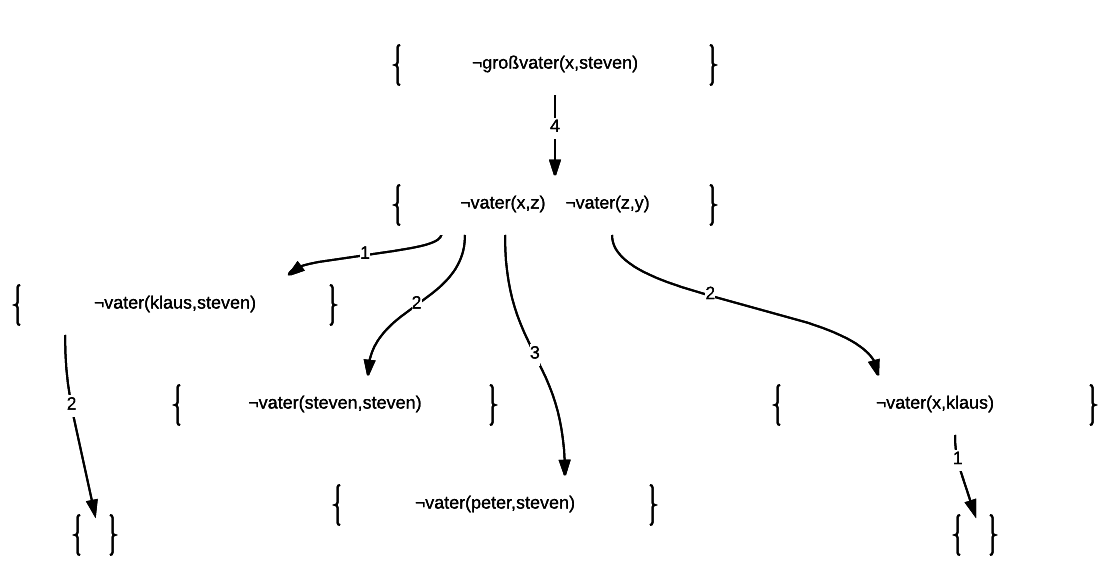
\includegraphics[scale=.9]{/home/steven/dev/lisp/cl-reason/doc/images/sld-tree.png}
	\caption{SLD-Baum}
	\label{sld-baum}
\end{figure}

Ein Resolutionsbeweis nach SLD-Strategie ist ein Wurzelpfad im SLD-Baum. Die SLD-Resolution ist widerlegungsvollständig für Mengen von Hornklauseln.

\chapter{Prolog}\label{prolog}
Die derzeit wichtigste logische Programmiersprache ist Prolog \cite{prolog}. Der rein logische Teil der Sprache besteht aus einem Schlussfolgerungssystem basierend auf der SLD-Resolution. Hinzu kommt ein nicht-logischer Teil, der es ermöglicht praktische Anwendungen rein in Prolog zu implementieren. Im folgenden wird der rein logische Kern von Prolog vorgestellt.

\section{Syntax}
Prologs Syntax entspricht weitgehend der Syntax der Prädikatenlogik, wobei nur Hornklauseln in Fakten- und Regelform zulässig sind.

Die Syntax für Terme entspricht Definition \ref{terme}. Zwischen Variablen und Konstanten wird dabei durch Groß- und Kleinschreibung unterschieden. Bezeichner die mit einem Großbuchstaben beginnen sind Variablen, alle anderen Bezeichner werden als Konstanten interpretiert.

Listen stellen eine Erweiterung der Terme wie sie in Kapitel \ref{logik} vorgestellt werden dar.

\begin{leftbar}
  \begin{definition}[Prologlisten]\label{prologlisten}
    \begin{description}
    \item[(IA_{1})] [] ist eine Liste (leere Liste)
    \item[(IA_{2})] Sind $t_{1}$ bis $t_{n}$ Terme, dann ist $[t_{1},...,t_{n}]$ eine Liste.
    \item[(IS)] Wenn $L$ eine Liste ist und $X$ ein Term, dann ist $[X|L]$ eine Liste.
    \end{description}
  \end{definition}
\end{leftbar}
\noindent
Mit den Operatoren {\tt :-} (entspricht $\Leftarrow$) und {\tt ,} (entspricht $\vee$) können nun aus Prädikaten Klauseln gebildet werden. Ein Punkt ({\tt .}) schließt eine Klausel ab.

Ein Beispiel für ein einfaches Prolog-Programm ist {\tt alle-kleiner}.

\begin{verbatim}
  alle-kleiner([],N).
  alle-kleiner([F|R],N) :- F < N, alle-kleiner(R,N). 
\end{verbatim}
\noindent

\section{Semantik}
Das Programm {\tt alle-kleiner} beschreibt eine Relation zwischen Listen von Zahlen und einer Zahl $n$, die jeweils erfüllt ist, wenn alle Elemente der Liste kleiner sind als $n$. Für das Schlussfolgerungssystem ist dieses Programm nun eine Menge geschlossener Formeln (durch universellen Abschluss). Stellt man nun die Anfrage

\begin{verbatim}
  alle-kleiner([1,3,5],6).
\end{verbatim}
\noindent
führt Prolog eine SLD-Resolution auf der Klauselmenge
\begin{flalign*}
\left \{ & \left \{ alle-kleiner(empty,x) \right \}^{1}, &\\
         & \left \{ alle-kleiner(cons(f,r),x), \neg <\left ( f,x \right ), \neg alle-kleiner(r,x) \right \}^{2}, &\\
         & \left \{ \neg alle-kleiner(cons(1,cons(3,cons(5,empty))),x) \right \}^{3} \left. \right \}
\end{flalign*}
\noindent
durch. Die ersten beiden Klauseln ergeben sich aus dem Programm und werden als Stützmenge gewählt. Die dritte Klausel ergibt sich aus der negierten Behauptung und steht bereits als Elternklausel für den ersten Resolutionsschritt fest. Nun wird gemäß der Selektionsfunktion eine passende Klausel zur Resolution mit der Zielklausel gewählt.

Die in Prolog verwendete Selektionsfunktion liefert dabei die gemäß der Reihenfolge im Programm erste Klausel, deren positives Literal sich mit dem ersten Literal der Zielklausel unifizieren lässt.

In der Resolvente stehen die neuen Teilziele aus der Programmklausel stets vor den Teilzielen aus der Zielklausel. Kann das erste Teilziel der Zielklausel nicht mit einem positiven Literal einer Programmklausel unifiziert werden, wird ein Backtracking eingeleitet. Dazu wird die aktuelle Zielklausel verworfen und damit auch alle Variablenbelegungen aus der letzten Unifikation zurückgenommen. Dann wird nach einer alternativen Unifikationsmöglichkeit für das erste Teilziel gesucht.

Ist das nächste Teilziel ein vordefiniertes Prädikat (wie z. B. {\tt <}), wird nicht nach einer passenden Zielklausel gesucht sondern eine Sonderbehandlung angestoßen, die eine neue Zielklausel liefert oder bei Nichterfüllung des Prädikats Backtracking auslöst.

Die Suchstrategie von Prolog entspricht aufgrund der Reihenfolge der Teilzielauswertung einer Tiefensuche im SLD-Baum.

\subsection{Unvollständigkeit von Prolog}
Die Resolution nach der SLD-Strategie ist ein nichtdeterministisches Verfahren. In jedem Schritt liegen unter Umständen mehrere Ableitungsmöglichkeiten abhängig von

\begin{itemize}
\item der gewählten Programmklausel und
\item des gewählten Teilziels
\end{itemize}

vor. Die in Prolog gewählte Selektionsfunktion und die forcierte Reihenfolge der Teilziele in der Zielklausel stellen zwar Determinismus sicher, sind aber auch Grund für die größte Schwäche von Prolog: die Unvollständigkeit des Schlussfolgerungssystems. \cite{beckstein}

Jedes erfolgreiche Blatt im SLD-Baum, das hinter einem unendlichen Wurzelpfad liegt, ist effektiv unerreichbar. Wir betrachten folgendes Prolog Programm aus \cite{lloyd}:

\begin{verbatim}
p(a,b).
p(c,b).
p(X,Z) :- p(X,Y), p(Y,Z). -- transitivität
p(X,Y) :- p(Y,X).         -- kommutativität
\end{verbatim}
\noindent
Theoretisch sollte das Schlussfolgerungssystem die Anfrage

\begin{verbatim}
p(a,c).
\end{verbatim}
\noindent
bejahen. Aufgrund der Selektionsfunktion wird Prolog jedoch stets eine Unifikation mit der dritten Klausel versuchen, da das positive Literal {\tt p(X,Z)} mit jeder Anfrage zum Prädikat {\tt p} unifizierbar ist. Für eine erfolgreiche Ableitung der leeren Klausel wird jedoch auch die vierte Klausel benötigt. Das Resultat ist ein Stackoverflow während der Lösungsfindung.

Die Lösung dieses Problems war nicht teil der Aufgabenstellung. Das in dieser Arbeit entwickelte Schlussfolgerungssystem leidet also unter derselben Schwäche.

\chapter{Konzeption}\label{konzeption}

In diesem Kapitel werden die entwickelten Grammatiken zur Beschreibung der Eingabesprache, die gewählte Methode zur Antwortbestimmung sowie die Algorithmen die das Schlussfolgerungssystem bilden beschrieben.

\section{Beschreibungssprache}
Das System verarbeitet Formeln definiert in einer formalen Sprache.

Zur Beschreibung der Sprache wurden zwei kontextfreie Grammatiken definiert, die jeweils eine Ebene der Sprache beschreiben. Auf der obersten Ebene werden Programme als Folge von Hornklauseln in Regel- oder Faktendarstellung betrachtet. Prädikate samt ihrer Argumente werden dabei als ein Eingabesymbol betrachtet. Dies wird durch eine vorherige lexikalische Analyse ermöglicht, die den Eingabestring in Tokens zerlegt, und dabei die Argumente von Prädikaten als Property in den erzeugten Literal-Symbolen speichert.

Auf der unteren Ebene werden Terme wie sie als Argumente von Prädikaten auftauchen geparst.

\subsection{Lexikalische Analyse}
Die Eingabe in den Lexer ist das vom Benutzer verfasste Programm als String. Mittels eines regulären Ausdrucks wird dieser String in die einzelnen Bausteine (sog. Tokens) des Programms zerlegt.

\begin{leftbar}
  \begin{definition}[CL-Reason Tokens]
    \newline
    Die in der lexikalischen Analyse zu identifizierenden Token sind Worte der Sprache
    \begin{flalign*}
      & \left \{ a,..,z \right \} \cup \left \{ forall,exists,and,<=,=>,:,. \right \} \cup \\
      & \left \{  w(t) \; | \; w \in \left \{ a,...,z,A,...,Z,0,...,9 \right \}^{*}, t \in \left \{a,...,z,0,...,9,(,),, \right \}^{*} \right \} 
    \end{flalign*}
  \end{definition}
\end{leftbar}

Es ist anzumerken, dass die zu matchende Sprache nicht regulär ist. Moderne Regex-Engiens erlauben jedoch das verwenden von Lookaheads, wodurch eine Erkennung von korrekt geklammerten Prädikatsdeklarationen möglich ist. Die in Abschnitt \ref{proggram} definierte Grammatik für Programme legt fest, dass auf ein Prädikat entweder eine Implikation, eine Konjunktion oder das Ende der Klausel folgen muss. Aufgrund dieser Tatsache lässt dich mittels eine Lookaheads entscheiden, ob eine schließende Klammer tatsächlich ein Prädikat abschließt, oder noch zur Liste der Terme innerhalb des Prädikats gehört.

\subsection{Grammatik für Programme}\label{proggram}
Auf der obersten Ebene besteht ein Programm aus einer Folge von Hornklauseln in Regel- oder Faktendarstellung.

\begin{leftbar}
  \begin{definition}[$G_{cl-reason}$]\label{proggramdef}
    \newline
    Die kontextfreie Grammatik $G_{cl-reason} = \left ( \Sigma,N,P,S \right )$ mit
    \begin{itemize}
    \item $\Sigma = \left \{ forall, exists, and, in, end, var, lit, <= , => \rigth \}$,
    \item $N = \left \{ S, V, K, F, F' \right \}$ und    
    \end{itemize}
    \begin{flalign*}
      P: S & \rightarrow forall\; VKS\; |\; exists\; VKS\; |\; lit\; end\; S\; |\; \epsilon &\\
      V & \rightarrow var\; V\; |\; var\; in &\\
      K & \rightarrow lit\; <=\; F\; |\; lit\; and\; F'\; |\; lit\; end &\\
      F & \rightarrow lit\; and\; F\; |\; lit\; end & \\
      F' & \rightarrow lit\; and\; F\; |\; lit\; =>\; lit\; end\;
    \end{flalign*}
    \noindent
    erzeugt alle gültigen Programme der Sprache CL-Reason
  \end{definition}
\end{leftbar}
\noindent
Das Alphabet $\Sigma$ enthält alle Token die in der vom Lexer erzeugten Ausgabe enthalten sein können. Ausgehend vom Startsymbol $S$ lässt sich eine beliebig lange Folge von Klauseln bestehend aus einer Variablendeklaration mit $forall$ oder $exists$ gefolgt von beliebig vielen Variablen und der eigentlichen Klausel in Fakt- oder Regeldarstellung erzeugen.

Mit dem Nichtterminal $V$ lässt sich eine beliebig lange Folge von Variablen erzeugen.

Das Nichtterminal $K$ leitet die Erzeugung einer Klausel in Regeldarstellung ein. Da sowohl links- als auch rechtsgerichtete Implikationen erlaubt sind, muss über die Unterscheidung zwischen den Nichtterminalen $F$ und $F'$ sichergestellt werden, dass Programme der Form

\begin{verbatim}
forall x: p(x) <= q(x) and s(x) => r(x).
\end{verbatim}
\noindent
nicht erzeugt werden können.

Die Frage nach der syntaktischen Korrektheit eines gegebenen Programms kann durch einen $LL(2)$ Parser beantwortet werden. Bei der Expansion eines Nichtterminal kann mit einem Lookahead von zwei Terminalsymbolen die zu wählende Produktion eindeutig bestimmt werden. Der Aufbau des Entwickelten Parser ist im Detail im Abschnitt \ref{progparser} beschrieben.

\subsection{Grammatik für Terme}
Ein Teil der Grammatik für Terme ergibt sich direkt aus der induktiven Definition von Termen aus Definition \ref{terme}. In CL-Reason wird für die Darstellung von Listen eine spezielle Syntax verwendet.

\begin{leftbar}
  \begin{definition}[Listen]
    \newline
    \begin{description}
    \item[(IA)] Die Konstante $empty$ ist eine Liste (leere Liste).
    \item[(IS)] Wenn $l$ eine Liste und $x$ eine Term ist, dann ist auch $cons(x,l)$ eine Liste.
    \end{description}
  \end{definition}
\end{leftbar}
\noindent
Mit dieser induktiven Definition lassen sich beliebige Listenstrukturen als Terme gemäß von Definition \ref{terme} darstellen. Da diese Darstellung zur Formulierung von geschachtelten Listen unhandlich ist, können in CL-Reason Listen in der aus Prolog bekannten Syntax formuliert werden (Definition \ref{prologlisten}).

Arithmetische Ausdrücke lassen sich in Infix-Notation formulieren. Dabei können die Operatoren $+$ (Addition), $-$ (Subtraktion), $*$ (Multiplikation) und $/$ (Division) verwendet werden. Des weiteren können arithmetische Ausdrücke beliebig geklammert werden.

\begin{leftbar}
  \begin{definition}[$G_{Terme}$]\label{termgram}
    \newline
    Die kontextfreie Grammatik $G_{Terme} = \left ( \Sigma,N,P,S \right )$ mit
    \begin{itemize}
    \item $\Sigma = \left \{ LB, RB, LS, CONS, LE, +, -, *, /, SEP, INT, SYM \rigth \}$,
    \item $N = \left \{ S, T, A, F, L \right \}$ und    
    \end{itemize}
    \begin{flalign*}
      P: S & \rightarrow LB\; T\; RB &\\
      T & \rightarrow SYM\; |\; A\; |\; L\; |\; T\; SEP\; T\; |\; \epsilon &\\
      A & \rightarrow A\; +\; A\; |\; A\; -\; A\; |\; A\; *\; A\; |\; A\; /\; A\; |\; LB\; A\; RB &\\
      F & \rightarrow  SYM\; LB\; T\; RB\; &\\
      L & \rightarrow LS\; T\; LE\; |\; LS\; SYM\; CONS\; SYM\; LE\; |\; LS\; SYM\; CONS\; L\; LE
    \end{flalign*}
    \noindent
    erzeugt alle gültigen Terme.
  \end{definition}
\end{leftbar}
\noindent
Terme werden durch einen Bottom-Up Parser, der direkt aus der Grammatik generiert wurde, geparst (siehe Abschnitt \ref{termparser}).

\section{Semantik}
Die Semantik von CL-Reason entspricht der Semantik von Prolog. Der SLD-Baum wird entsprechend einer Tiefensuche nach einem Blatt durchsucht.

Zur Bestimmung einer erfüllenden Variablenbelegung wird ein Antwortprädikat verwendet.

\begin{leftbar}
  \begin{definition}[Antwortprädikat]
    \newline
    Ein Antwortprädikat ist ein zu einer Zielklausel hinzugefügtes, positives Literal, das als Argumente alle in der Zielklausel vorkommenden Variablen enthält.
  \end{definition}
\end{leftbar}
\noindent
Aus der Anfrage
\begin{verbatim}
exists x y: p(x,y).
\end{verbatim}
\noindent
entsteht also die initiale Zielklausel $\left \{ \neg p(x,y), answer(x,y) \rigth \}$.

Da bei der SLD-Resolution an jedem Resolutionsschritt eine Goalklausel beteiligt ist, ist immer auch ein Antwortprädikat beteiligt. Das Ziel der Resolution ist nun nicht mehr die leere Klausel abzuleiten, sondern eine Klausel die nur noch das Antwortprädikat enthält. Die erfüllende Variablenbelegung kann dann in der Argumentliste des Antwortprädikats abgelesen werden.

\section{Algorithmen}
Die zentrale Operation des Schlussfolgerungssystems ist die Unifikation von Literalen. In jedem Schritt der Lösungsfindung legt die SLD-Strategie fest, zwischen welchen Klauseln eine Unifikation durchgeführt werden soll, und was bei Nichterfolg zu tun ist.

In diesem Schritt werden der verwendete Unifikationsalgorithmus sowie der Resolutionsalgorithmus nach SLD-Strategie beschrieben.

\subsection{Unifikationsalgorithmus}\label{unialg}
Die Unifikation von Literalen wurde im Abschnitt \ref{res} auf die Unifikation von Termen zurückgeführt. Der verwendete Unifikationsalgorithmus ist eine rekursive Variante des Unifikationsalgorithmus für Termlisten nach \cite{Robinson}.

Wir betrachten zunächst die Komposition zweier idempotenter Substitutionen.

\begin{leftbar}
  \begin{definition}[Komposition von Substitutionen]
    \newline
    Seien
    \begin{eqnarray}
      \sigma = \left \{ x_1 \leftarrow s_1,...,x_n \leftarrow s_n\right \} \\
      \tau = \left \{ y_1 \leftarrow t_1,...,y_m \leftarrow t_m \right \}
    \end{eqnarray}
    zwei Substitutionen, sodass
    \begin{equation}
      \left \{ x_1,...,x_n\right \} \cap \left \{ y_1,...,y_m\right \} = \emptyset
    \end{equation}
    Dann ist
    \begin{equation}
      \sigma \circ \tau = \left \{ x_1 \leftarrow \tau s_1,...,x_n \leftarrow \tau s_n \right \} \cup \tau
    \end{equation}
  \end{definition}
\end{leftbar}
\noindent
Der folgende Algorithmus liefert den mgu für zwei Termlisten $s = (s_1,...,s_n)$ und $t = (t_1,...,t_n)$.

\begin{small}
\[ unify(s,t,\sigma)=_{def}
  \begin{cases}
    \sigma    & \quad length(s) = length(t) = 0\\
    unify(rest(s),rest(t),\sigma) & \quad \sigma s_1 = \sigma t_1\\
    unify(rest(s),rest(t),\sigma \circ \left \{ \sigma s_1 \leftarrow \sigma t_1 \right \})  & \quad \sigma s_1 \text{ oder } \sigma t_1 \text{ ist Variable (o.B.d.A sei }\\
    & \quad \sigma s_1 \text{ Variable) und } \sigma s_1 \text{ kommt nicht in } \sigma t_1 \text{ vor}\\
    unify(rest(s),rest(t),\sigma \circ \tau)  & \quad \sigma s_1 = f(x_1,...,x_m) \text{ und } \sigma t_1 = (y_1,...,y_m) \\
    & \quad \text {und } \tau = unify((x_1,...,x_m)(y_1,...,y_m),\left \{ \right \}) \neq fail\\
    fail & \quad \text{sonst}
  \end{cases}
  \]
\end{small}

\subsection{SLD-Resolutionsalgorithmus}\label{sld-res}
Wie bereits im Kapitel \ref{prolog} beschrieben, ist eine extreme Einschränkung der Auswahlmöglichkeiten in jedem Resolutionschritt nötig, um die SLD-Resolution deterministisch implementierbar zu machen. Auch in diesem System werden Programmklauseln anhand ihrer Position im Programm ausgewählt. Neu entstandene Teilziele werden vorne in die Resolvente eingefügt und direkt im nächsten Resolutionsschritt bearbeitet. Der Algorithmus entspricht also einer Tiefensuche im SLD-Baum.

Wir entwickeln den Algorithmus anhand eines Beispiels. Sei folgendes CL-Reason Programm gegeben.

\begin{verbatim}
q(3).
s(4).
p([]).
forall f r: p([f|r]) <= q(f) and p(r).
forall f r: p([f|r]) <= s(f) and p(r).
\end{verbatim}
\noindent

Anfragen an das Prädikat {\tt p} liefern {\tt true}, wenn alle Elemente der als Argument übergebenen Liste entweder Dreien oder Vieren sind. Wird nun die Anfrage

\begin{verbatim}
p([3,4]).
\end{verbatim}
\noindent

gestellt, wird eine SLD-Resolution auf der Klauselmenge

\begin{flalign*}
\left \{ & \left \{ q(3) \right \}^{1}, &\\ 
         & \left \{ s(4)\rightt \}^{2}, &\\ 
         & \left \{ p(empty) \right \}^{3}, &\\
         & \left \{ p(cons(f,r), \neg q(f), \neg p(r) \right \}^{4}, &\\
         & \left \{ p(cons(f,r), \neg s(f), \neg p(r) \right \}^{5}, &\\
         & \left \{ \neg p(cons(3,cons(4,empty))) \right \}^{6} \rigth \}
\end{flalign*}
\noindent
angestoßen. Klausel sechs ist dabei die erste Zielklausel.

Wie in der Tiefensuche üblich, werden die zu expandierenden Knoten auf einen Stack gelegt. Da das erzeugen von Resolventen der aufwendigste Schritt in diesem Algorithmus ist, wird immer nur eine Resolvente erzeugt und diese direkt als neue Goalklausel betrachtet. 

Um an jedem inneren Knoten des Baumes die nächste Ableitung bestimmen zu können, werden die potenziell zum ersten Teilziel passenden Programmklauseln auf einem Stack gelegt. Wir bezeichnen diesen Stack als aktuelle Prozedur. Diese Prozedur wird dann auf einen Stack von Prozeduren gelegt, dessen Zweck nach dem nächsten Schritt deutlich wird. Abbildung \ref{algostate1} zeigt die Startkonfiguration.

\begin{figure} %[hbtp]
	\centering
		\includegraphics[scale=.9]{/home/steven/dev/lisp/cl-reason/doc/images/algostate_1.png}
	\caption{Startkonfiguration des Algorithmus}
	\label{algostate1}
\end{figure}

Nun werden der Reihe nach Unifikationen mit den Programmklauseln der aktuellen Prozedur versucht. Die erste erfolgreiche Unifikation findet mit Klausel vier statt. Die daraus resultierende Resolvente wird auf den Stack der Goalklauseln gelegt. Sollte eines der Teilziele in dieser Goalklausel nicht gelöst werden können, gelangen wir durch Backtracking (entfernen von Goalklauseln vom Stack) wieder zur ersten Goalklausel. An dieser Stelle muss bekannt sein, mit welchen Programmklauseln bereits eine Unifikation versucht wurde. Zu diesem Zweck legen wir die aktuelle Prozedur auf einen Stack. Auf diesen Stack wird nach der Ableitung einer neuen Klausel auch direkt die zum ersten Teilziel der Resolvente passende Prozedur gelegt. Die Abbildung \ref{algostate2} verdeutlicht die neue Konfiguration.

\begin{figure} %[hbtp]
	\centering
		\includegraphics[scale=.9]{/home/steven/dev/lisp/cl-reason/doc/images/algostate_2.png}
	\caption{Konfiguration nach der ersten Ableitung}
	\label{algostate2}
\end{figure}

Nun werden erneut Unifikationen zwischen dem ersten Teilziel $\neg q(3)$ und den Programmklauseln der obersten Prozedur versucht. Dies gelingt und es entsteht die Resolvente $\left \{ \neg p(cons(4,empty))\right \}$. Die neue Zielklausel wird auf den Stack der Zielklauseln gelegt und die zum ersten Teilziel $\neg p(cons(4,empty))$ passende Prozedur wird auf den Prozedurenstack gelegt.

Dieses Verfahren wird fortgesetzt, bis es zur in Abbildung \ref{algostate3} gezeigten Situation kommt.

\begin{figure} %[hbtp]
	\centering
		\includegraphics[scale=.9]{/home/steven/dev/lisp/cl-reason/doc/images/algostate_3.png}
	\caption{Konfiguraton vor erstem Backtracking}
	\label{algostate3}
\end{figure}

Das durch die Resolution der Klauseln acht und vier eingeführte Teilziel $\neg q(4)$, kann nicht durch die Programmklauseln in der obersten Prozedur gelöst werden. Eine leere Prozedur auf dem Prozedurenstack ist das Signal zum Backtracking, da dies nur in Situationen auftritt, in denen ein Teilziel nicht durch das Programm gelöst werden kann. Nun wird sowohl die oberste Prozedur als auch die oberste Goalklausel verworfen und das Verfahren mit den neuen obersten Objekten beider Stacks vorgesetzt. Als nächstes wird also nach einer alternativen Ableitung für Klausel acht gesucht. Dies gelingt mit der Klausel fünf und es entsteht die Situation in Abbildung \ref{algostate4}.

\begin{figure} %[hbtp]
	\centering
		\includegraphics[scale=.9]{/home/steven/dev/lisp/cl-reason/doc/images/algostate_4.png}
	\caption{Konfiguraton nach finden einer alternativen Ableitung}
	\label{algostate4}
\end{figure}

Nun kann das Verfahren ohne weiteres Backtracking fortgesetzt werden. Durch die zweite Klausel kann das Teilziel $\neg s(4)$ aufgelöst werden und durch Klausel drei schließlich das Teilziel $\neg p(empty)$. Der Algorithmus bricht mit {\tt FAIL} ab, wenn der Prozedurenstack leer ist.

Die Implementierung dieses Verfahren stellt den Kern des Schlussfolgerungssystems dar.

\chapter{Implementierung}\label{implementierung}

In diesem Kapitel wird auf Implementierungsdetails des Parsers und die durch ihn erzeugte interne Repräsentation von Formeln eingegangen. Der Unifikationsalgorithmus und das Resolutionsverfahren wurden bereits in Kapitel \ref{konzeption} ausführlich beschrieben. Die Implementierung dieser beiden Algorithmen wird nicht näher beschrieben.

\section{Lexing und Parsing}
Geparst werden Programme aus einer einfachen Textdatei. Im ersten Schritt wird der Eingabetext durch einen regulären Ausdruck in Tokens zerlegt (das sog. lexing). Der reguläre Ausdruck wurde mit der Library cl-ppcre \cite{cl-ppcre} erstellt. Die Syntax für reguläre Ausdrücke in dieser Library entspricht der Syntax von Perl.

\begin{verbatim}
forall|exists|and|<=|=>|:|[a-zA-Z0-9]+\\(.*\\)(?=\\s*<=)
|[a-zA-Z0-9]+\\(.*\\)(?=\\s*and)|[a-zA-Z0-9]+\\(.*\\)(?=\\s*=>)
|[a-zA-Z0-9]+\\(.*\\)(?=\\.)|[a-z]+|\\.
\end{verbatim}

Die ersten sechs Fälle entsprechen vordefinierten Schlüsselwörtern. Die nächsten vier Fälle matchen Prädikatsdefinitionen. Das Ende einer Prädikatsdefinition (die letzte schließende Klammer) wird über einen Lookahead identifiziert. So wird eine Prädikatsdefinition nur dann gematcht, wenn auf sie entweder {\tt <=}, {\tt and}, {\tt =>} oder {\tt .} folgt.

Nachdem der Eingabetext so in Schlüsselwörter und Prädikatsdefinitionen zerlegt wurde, werden für Prädikatsdefinitionen Symbole angelegt und der Name sowie die Argumentenliste in Properties gespeichert. Die Argumentenliste liegt nach diesem Schritt noch als String vor und muss in einem späteren Schritt durch den Termparser geparst werden (Abschnitt \ref{termparser}). Auch für Variablen werden Symbole angelegt, die nach dem Parsen der Terme an den entsprechenden Stellen in die Terme eingefügt werden. So ist sichergestellt, dass die Variablen innerhalb einer Klausel eindeutig, von Klausel zu Klausel jedoch unterschiedlich sind.

\subsection{Parser für Programme}\label{progparser}
Der erste Parser stellt fest, ob die vom Lexer erzeugte Folge von Tokens ein gültiges Programm ist. Es handelt sich dabei um einen $LL(2)$-Parser, da die Eingabe von links nach rechts abgearbeitet wird und anhand eines Lookaheads von zwei Terminalsymbolen eine Ableitung für das am weitesten Links stehende Nichtterminal ausgewählt wird. Geparste Prädikatssymbole werden je nach Position im Programm als positives oder negatives Literal einer Klausel interpretiert und in entsprechenden Properties eines Klauselsymbols gespeichert.

Der Parser ist in mehrere Funktionen aufgeteilt. Gesteuert wird das Parsing in der  Hauptfunktion {\tt parse-program}, die die als nächstes zu expandierenden Nichtterminale, die schon teilweise geparste Tokenfolge sowie die bereits erstellte Klauselmenge verwaltet.

\begin{verbatim}
(defun parse-program (input)
  (do* ((ntl '(s)) ;; Liste der Nichterminale, zu Beginn zur s
       (program input)
       (output NIL)
       (la (take 2 program) 
           (take 2 program)) 
               ;; zwei Terminalsymbole als Lockahead
       (expansion (funcall (next-nt ntl) la) 
                  (funcall (next-nt ntl) la))
               ;; Aufruf der Funktion zum am weitesten 
               ;; links stehenden Nichtterminal
       (production (nth 2 expansion) (nth 2 expansion))
               ;; Zahlencode der gewählten Ableitung
       (to-match (car expansion) (car expansion))
               ;; zu matchende Terminalsymbole
       (new-nt (cadr expansion) (cadr expansion)))
               ;; als nächstes zu expandierende Nichtterminale
    ((and (not program) (not ntl)) (reverse output))
         ;; Abbruchbedingung
    (case production
      ...
      ;; Erweiterung des Output je nach Produktion
      ...
      )
    (setq program (match (car expansion) program))  
            ;; konsumieren der Eingabe von links
    (setq ntl (append new-nt (cdr ntl)))
            ;; erweitern der Nichtterminalliste))
\end{verbatim}

Das expandieren von Nichtterminalen wird anhand eines Lookaheads von gesonderten Funktionen übernommen. Dabei gibt es für jedes Nichtterminal eine Funktion, die anhand des Lookaheads entscheidet, welche Terminalsymbole als nächstes gematcht werden können und welche Nichtterminale als nächstes expandiert werden müssen. Die Regeln nach denen diese Nichtterminalfunktionen arbeiten ergeben sich aus der Grammatik aus Definition \ref{proggramdef}. Wir betrachten hier beispielhaft die Funktion zum Nichtterminal {\tt S}.
\newpage

\begin{verbatim}
(defun s (la)
  (cond ((la-check la '(forall var))
         '((forall) (v k s) 0))
        ((la-check la '(exists var))
         '((exists) (v k s) 1))
        ((la-check la '(lit end))
          '((lit end) (s) 2))
        ((la-check la NIL)
         '(nil nil 3))
        (T (error "no fitting production"))))
\end{verbatim}

Die Funktion erhält aus der Hauptfunktion die nächsten zwei Symbole der Eingabe als Parameter {\tt la}. Die Funktion {\tt la-check} liefert true, falls der Wert der Symbole in {\tt la} den Symbolen im zweiten Argument entsprechen. Diese Funktion ist notwendig, das z. B. die Literaltokens in der Eingabe des Parsers durch den Lexer bereits mit Propertys versehen sind.

Passt der Lookahead zu einer möglichen Produktion wird ein Trippel zurückgeliefert. Das erste Element dieses Trippels ist eine Liste mit Terminalsymbolen, die nun durch die Hauptfunktion gematcht werden können. Die Anzahl der Terminalsymbole ist Situationsbedingt. Ist es anhand des Lookahead möglich mehr als ein oder zwei Terminalsymbole zu matchen so wird dies auch getan.

Das zweite Element des Trippels ist eine Liste mit Nichtterminalen, die als nächstes zu expandieren sind. Diese Liste wird in der Hauptfunktion vorne an die Liste der als nächstes zu expandierenden Nichtterminale angefügt.

Das letzte Element des Trippels ist ein Zahlencode, der die in der Hauptfunktion auszuführenden Aktionen beschreibt. Je nach Antwort der Nichtterminalfunktion werden dann in der Hauptfunktion die nötigen Aktionen angestoßen. Dazu gehören das Anlegen einer neuen Klausel beim Parsen eines Quantors, das Hinzufügen von geparsten Variablensymbolen zur Liste von Variablen einer Klausel oder das setzen eins geparsten Literals als positives oder negatives Literal einer Klausel. So wird bereits beim Parsen eine gewisse Interpretation der Eingabe vorgenommen, die sich in der internen Repräsentation der Daten widerspiegelt.

Die interne Struktur eines geparsten Programms wie sie vom Parser erzeugt wird entspricht der Abbildung \ref{internrep1}

\begin{figure} %[hbtp]
	\centering
		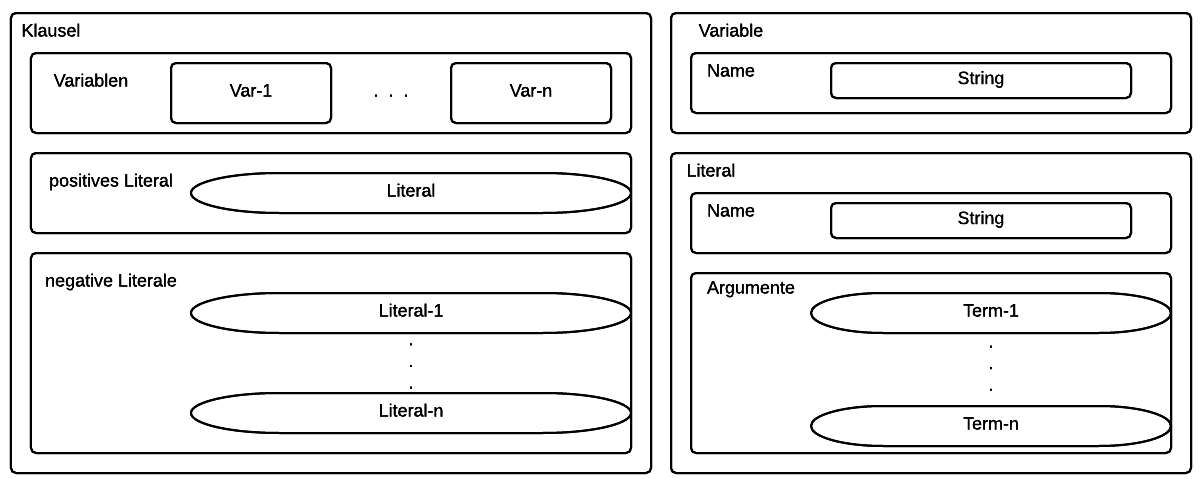
\includegraphics[scale=.7]{/home/steven/dev/lisp/cl-reason/doc/images/internrep1.png}
	\caption{interne Repräsentation von Programmen}
	\label{internrep1}
\end{figure}

\subsection{Parser für Terme}\label{termparser}
Der Parser für Terme wurde durch einen Parsergenerator direkt aus der Grammatik aus Definition \ref{termgram} generiert. Verwendet wurde die Parsergenerator Library cl-yacc \cite{cl-yacc}. Der Erzeugte Parser arbeitet auf einer Folge von Tokens die aus den in Properties der Literale gespeicherten Strings erzeugt werden.
\newpage

\begin{verbatim}
(defun tokenize-terms (termstring)
  (mapcar (lambda (x)
            (cond ((string= x "(") 'LB)
                  ((string= x ")") 'RB)
                  ((string= x "[") 'LS)
                  ((string= x "|") 'CONS)
                  ((string= x "]") 'LE)
                  ((string= x "+") '+)
                  ((string= x "-") '-)
                  ((string= x "*") '*)
                  ((string= x "/") '/)
                  ((string= x ",") 'SEP)
                  ((cl-ppcre:scan "\\d+" x) (parse-integer x))
                  (T (read-from-string x))))
	  (remove " " (all-matches-as-strings *regex-term* termstring) 
                  :test 'string=)))
\end{verbatim}

Auch bei diesem Parser werden nach dem Parsen eines Teils der Eingabe bestimmte Operationen ausgeführt, die die geparsten Terme in eine interne Repräsentation überführen.

\section{Interpreter}
Nachdem ein Großteil der für die Resolution benötigten Informationen bereits durch die Parser in einer geeigneten internen Repräsentation gespeichert wurde, sind nur noch Terme, insbesondere Listen gesondert zu interpretieren.

Da für jede Klausel explizit angegeben werden muss, welche Symbole Variablen sind und für jede Variable bereits durch den Lexer ein Symbol angelegt wurde, müssen lediglich alle Vorkommnisse dieses Symbols in allen Termen einer Klausel durch das bereits existierende Variablensymbol ersetzt werden.

\subsection{Listen}
Der Termparser unterscheidet zwischen konkreten Listen der Form $[t_1,...,t_n]$ und abstrakten Listen der Form $[x|y]$. Für abstrakte Listen kann direkt eine entsprechende Darstellung als Term $cons(x,y)$ abgelesen werden.

Konkrete Listen müssen in einem gesonderten Schritt in diese Form überführt werden. Dazu wird rekursiv aus den geparsten Elementen der Liste ein Funktionsterm erzeugt.

Aus der Liste $[1,2,3,4]$ wird so der Funktionsterm

\begin{equation}
  cons(1,cons(2,cons(3,cons(4,empty))))
\end{equation}

Abbildung \ref{internrep2} zeigt die finale interne Repräsentation von Termen.

\begin{figure} %[hbtp]
	\centering
		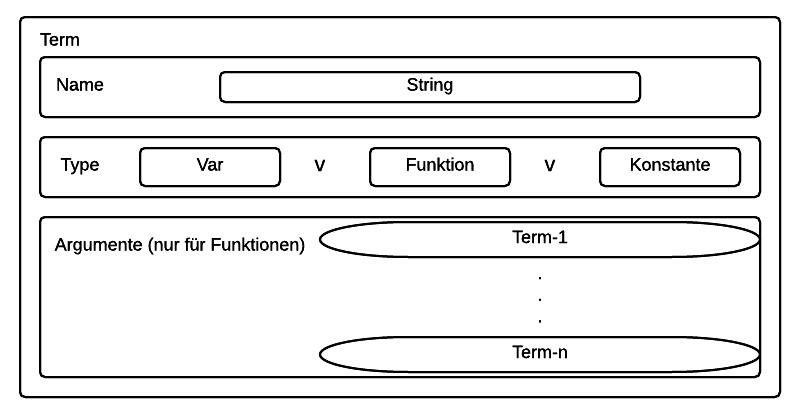
\includegraphics[scale=.9]{/home/steven/dev/lisp/cl-reason/doc/images/internrep2.png}
	\caption{interne Repräsentation von Termen}
	\label{internrep2}
\end{figure}
  
\section{Logisches Schlussfolgern}
Die beiden Kernfunktionen für die Implementierung des Schlussfolgerungssystems sind die Implementierungen des Unifikationsalgorithmus und des SLD-Resolutionsalgorithmus.

Die im Abschnitt \ref{unialg} angegebene rekursive Funktion zur Unifikation von Termlisten wurde rekursiv implementiert. Erweitert auf Literale wird sie während der SLD-Resolution verwendet.

\begin{verbatim}
(defun unify-literals (lit1 lit2) 
  (let ((name1 (get lit1 'name))
        (name2 (get lit2 'name))
        (args1 (mapcar 'copy-term-symbol (get lit1 'args)))
        (args2 (mapcar 'copy-term-symbol (get lit2 'args))))
    (if (and (string= name1 name2)
             (= (length args1)
                (length args2))) 
        (unify-termlists args1 args2 '())
       'fail)))
\end{verbatim}

Da die Anwendung von Substitutionen Teil des Algorithmus ist, ist es nötig, dass während der Unifikation lediglich auf Kopien der Termlisten gearbeitet wird. 

Das im Abschnitt \ref{sld-res} beschriebene Verfahren wurde als iterativer Algorithmus in der Funktion{\tt sld-resolution} implementiert.

Gestartet werden können Programme nach dem Laden des Systems durch einen Aufruf der Funktion {\tt run-program}. Als Argument erhält diese Funktion den Dateipfad des Programms. Da Anfragen direkt mit im Programm stehen, müssen sie durch einen Existenzquantor eingeleitet werden, auch wenn keine Variablen in der Anfrage vorkommen.

\chapter{Ausblick}\label{ausblick}
Das entwickelte System stellt lediglich den logischen Kern eines Schlussfolgerungssystem f{\"u}r Hornklauseln dar. In diesem Kapitel sollen kurz denkbare und sinnvolle Erweiterungen dargestellt werden.

\subsection*{User Interface}
Aktuell liegt das Schlussfolgerungssystem lediglich als Lisp Code vor, der in einem Lispsystem geladen werden kann. Programme k{\"o}nnen dann durch einen Aufruf der Funktion {\tt run-program} {\"u}ber Angabe des Pfades ausgewertet werden. Ein User Interface zum laden von Programmen und interaktivem Stellen von Anfragen w{\"a}re eine sinnvolle Erweiterung. Dadurch k{\"o}nnte auch das Problem der unn{\"o}tigen existenzquantifizierten Variablen in Anfragen gel{\"o}st werden.

\subsection*{Vordefinierte Pr{\"a}dikate}
Zahlen und arithmetische Ausdr{\"u}cke erf{\"u}llen bisher keinen besonderen Zweck. Zahlen werden als Konstanten und arithmetische Ausdr{\"u}cke als Funktionsterme interpretiert. Eine gesonderte Verarbeitung {\"u}ber vordefinierte Pr{\"a}dikate sollte leicht in die bestehenden Algorithmen einzubauen sein.

\subsection*{Sorten f{\"u}r Terme}
Funktionsterme sind als Symbole realisiert. Dies erm{\"o}glicht eine beliebige Erweiterung um Propertys. So k{\"o}nnte z. B. jedem Term eine Sorte zugewiesen werden.

\chapter{Zusammenfassung}
Im Zuge dieser Arbeit ist ein Schlussfolgerungssystem für Hornklauselmengen entstanden. Einfache logische Schlüsse werden durch das System bereits gezogen, zum vollständigen Ersatz von Prolog in der Lehrveranstaltung Angewandte Logik ist es jedoch noch nicht geeignet.

Das Auswerten von arithmetischen Ausdrücken durch vordefinierte Prädikate oder das Vergleichen von Zahlen ist noch nicht möglich. Viele der Übungsaufgaben der Veranstaltung erfordern allerdings diese Möglichkeiten.

Dennoch ist durch den Parser und durch die implementierten Verfahren eine gute Grundlage geschaffen worden, die direkt auf den theoretischen Grundlagen der Logik und Informatik aufbaut. Die Grundlagen der logischen und symbolischen Programmierung sowie Rekursion über Listen lassen sich bereits jetzt mit dem System üben.

Die gewählte interne Repräsentation von Formeln ermöglicht eine einfache Erweiterung und Weiterentwicklung des Systems.

% ...
%--------------------------------------------------------------------------
\backmatter                        		% Anhang
%-------------------------------------------------------------------------
\bibliographystyle{geralpha}			% Literaturverzeichnis
\bibliography{literatur}     			% BibTeX-File literatur.bib
%--------------------------------------------------------------------------
\printindex 							% Index (optional)
%--------------------------------------------------------------------------
\begin{appendix}						% Anh�nge sind i.d.R. optional
   %\chapter{Glossar}

\abbreviation{DisASTer}		{DisASTer (Distributed Algorithms Simulation Terrain), A platform for the Implementation of Distributed Algorithms}
\abbreviation{DSM}			{Distributed Shared Memory}
\abbreviation{AC}			{Linearisierbarkeit (atomic consistency)}
\abbreviation{SC}			{Sequentielle Konsistenz (sequential consistency)}
\abbreviation{WC}			{Schwache Konsistenz (weak consistency)}
\abbreviation{RC}			{Freigabekonsistenz (release consistency)}
			% Glossar   
   \chapter{Erkl{\"a}rung des Kandidaten}

Die Arbeit habe ich selbstst{\"a}ndig verfasst und keine anderen als die angegebenen Quellen- und Hilfsmittel verwendet.

\vspace{2cm}

\begin{minipage}[t]{3cm}
\rule{3cm}{0.5pt}
Datum
\end{minipage}
\hfill
\begin{minipage}[t]{9cm}
\rule{9cm}{0.5pt}
Unterschrift des Kandidaten
\end{minipage}
	% Selbstst�ndigkeitserkl�rung
\end{appendix}

\end{document}
